\documentclass{beamer}

\usepackage[utf8x]{inputenc}
\usepackage{graphicx}
\usepackage{german}

% paar Farben fuer listings
\usepackage{color}
\definecolor{javared}{rgb}{0.6,0,0} % for strings
\definecolor{javagreen}{rgb}{0.25,0.5,0.35} % comments
\definecolor{javapurple}{rgb}{0.5,0,0.35} % keywords
\definecolor{javadocblue}{rgb}{0.25,0.35,0.75} % javadoc

% quellcode
\usepackage{listings}
\lstset{language=Java,
basicstyle=\ttfamily\tiny,
keywordstyle=\color{javapurple}\bfseries,
stringstyle=\color{javared},
commentstyle=\color{javagreen},
morecomment=[s][\color{javadocblue}]{/**}{*/},
numbers=none,
numberstyle=\tiny\color{black},
stepnumber=2,
numbersep=10pt,
tabsize=4,
showspaces=false,
showstringspaces=false,
showtabs=false,
}

% sections als zwischenseite mit titel
\AtBeginSection[]{
  \begin{frame}
  \vfill
  \centering
  \begin{beamercolorbox}[sep=8pt,center,shadow=true,rounded=true]{title}
    \usebeamerfont{title}\insertsectionhead\par
  \end{beamercolorbox}
  \vfill
  \end{frame}
}

% blaue Links mit \href{link}{text}
\usepackage{hyperref}
\hypersetup{colorlinks=true, urlcolor=blue}

\usetheme{Boadilla}
\usecolortheme[named=red]{structure}

\beamertemplatenavigationsymbolsempty

\begin{document}

\title{Datenstrukturen in Java}
\subtitle{Datenstrukturen und Algorithmen im JDK}
\author{Andreas Klipp,\, \\Stephan Prätsch}
\institute{}
\date{\today} 
\logo{
\includegraphics[width=1cm]{logo_mercateo}}
\titlegraphic{
\includegraphics[width=2cm]{logo_mercateo}}

\frame{\titlepage}
\frame{\frametitle{Inhaltsverzeichnis}\tableofcontents} 

\section{Einleitung}

\frame{\frametitle{Einleitung}
\begin{center}
Warum das alles
\end{center}
}

\frame{\frametitle{Stark gekürzte Übersicht}
\begin{center}
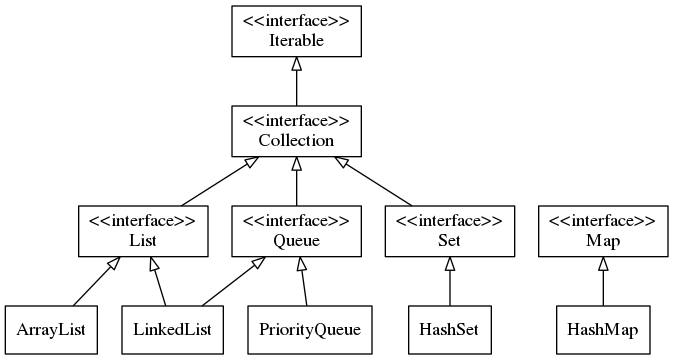
\includegraphics[width=0.9\textwidth]{java_util_overview_short}
\end{center}
}


\section{java.util.List}
\frame{\frametitle{java.util.List}
\begin{center}
Listen
\end{center}
}

\section{java.util.Map}
\frame{\frametitle{java.util.Map}
\begin{center}
Maps
\end{center}
}

\section{java.util.Queue}
\frame{\frametitle{java.util.Queue}
\begin{center}
Queues
\end{center}
}

\section{java.util.Set}
\frame{\frametitle{java.util.Set}
\begin{center}
Sets
\end{center}
}

\section{Hilfsfunktionen}

\begin{frame}[fragile]
  \frametitle{Hilfsfunktionen für Listen}
  \begin{block}{java.util.Collections.emptyList()}
    \begin{lstlisting}
      List<String> l = Collections.emptyList();
    \end{lstlisting}
  \end{block}
  \pause
  \begin{block}{com.google.common.collect.Lists.newArrayList(T...)}
    \begin{lstlisting}
      List<String> l = Lists.newArrayList("a", "b", "c", "d");
    \end{lstlisting}
  \end{block}
  \pause
  \begin{block}{java.util.AbstractList.subList(int, int)}
    from-index inklusiv, to-index exklusiv
    \begin{lstlisting}
      List<String> l = ...
      List<String> sub = l.subList(2,5);
    \end{lstlisting}
  \end{block}
  \pause
  \begin{block}{java.util.Collections.unmodifiableList(List\textless? extends T\textgreater)}
    \begin{lstlisting}
      Collections.unmodifiableList(list).add("a"); // wirft UnsupportedOperationException
    \end{lstlisting}
  \end{block}
\end{frame}
\begin{frame}[fragile]
  \frametitle{Hilfsfunktionen für Listen}
  \begin{block}{java.util.Collections.singletonList(T)}
    \begin{lstlisting}
      List<String> list = Collections.singletonList("a");
    \end{lstlisting}
  \end{block}
  \pause
  \begin{block}{java.util.Collections.synchronizedList(List\textless T\textgreater)}
    wrappt eine nicht synchronisierte List
    \begin{lstlisting}
      List<String> l = ...
      List<String> s = Collections.synchronizedList(l);
    \end{lstlisting}
  \end{block}
\end{frame}


\section{Abschluss}

\frame{\frametitle{Abschluss}
\begin{center}
Warum das alles
\end{center}
}

\frame{\frametitle{Stark gekürzte Übersicht}
\begin{center}
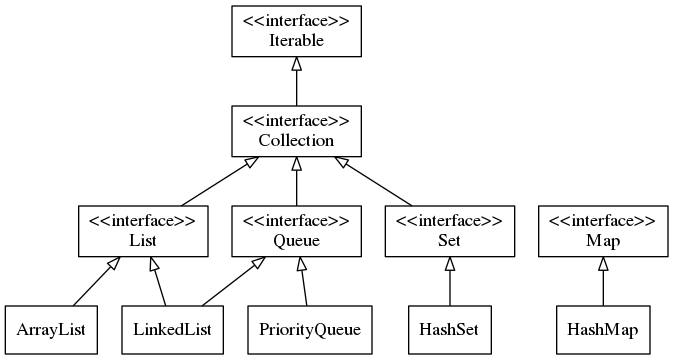
\includegraphics[width=0.9\textwidth]{java_util_overview_short}
\end{center}
}


\frame{\frametitle{Leicht gekürzte Übersicht}
\begin{center}
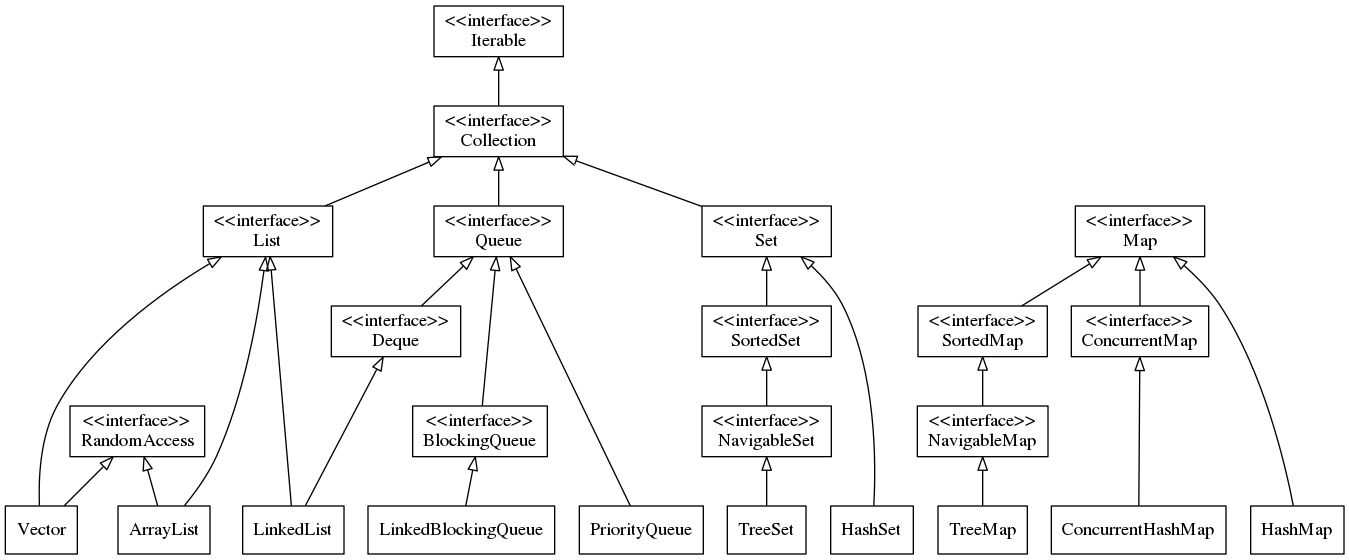
\includegraphics[width=0.9\textwidth]{java_util_overview}
\end{center}
}



\end{document}
